\documentclass[12pt]{article}
\usepackage[top=3cm, bottom=3cm, right=3cm, left=3cm]{geometry}
\usepackage{graphicx}
\usepackage{amsmath}
\usepackage{ulem}
\usepackage[english]{babel}
\usepackage[utf8]{inputenc}
\usepackage[T1]{fontenc}
\usepackage{hyperref}
\usepackage{bbold}
\usepackage{caption}
\usepackage{subcaption}
\usepackage{float}
\captionsetup[subfigure]{labelformat = parens, labelsep = space, font = small}


\begin{document}
\title{FYS3150 - Project 5 - Diffusion of neurotransmitters in the synaptic cleft}
\author{Vilde Flugsrud - Candidate number
\\ Mari Dahl Eggen - Candidate number 5}

\maketitle

\newpage

\tableofcontents

\newpage

\begin{flushleft}
\begin{abstract}
In this project we are analyzing the quality of five numerical procedures for solving partial differential equations. The equation of interest is the diffusion equation, and the numerical methods we are testing are Forward Euler, Backward Euler, Crank-Nicolson, and Monte Carlo with and without importance sampling. We will see that
\end{abstract}

\section{Introduction}
Neurotransmitters are information carrying molecules that are used in transport of signals between neurons in the brain. They are transported from a presynaptic cell to a postsynaptic cell, across a synaptic cleft, which is the small space that separates the cell membranes of the two cells. In Figure \ref{fig:cell} the cells and synaptic cleft are illustrated. In this project we are interested in how the neurotransmitters are moving across the synaptic cleft. We assume that they move due to diffusion, and will therefore solve the diffusion equation to figure out how the system evolves with time. The diffusion equation is a partial differential equation, and it exists many numerical methods for solving it. The equation is in this case also analytically solvable, which makes it easy to analyze the quality of the numerical methods. In this project we will test five different numerical methods, and compare the results from each, to determine which of the methods is the best.  

\begin{figure}[!h]
\begin{center}
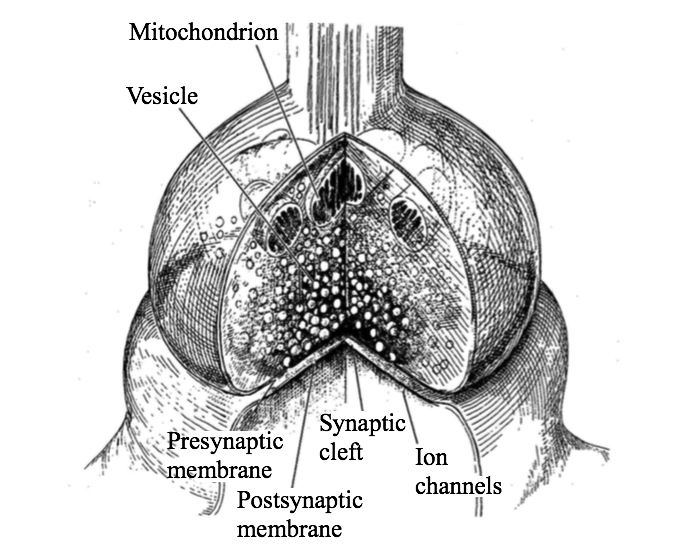
\includegraphics[scale=0.35]{cell2}
\caption{\label{fig:cell}Illustration of how the presynaptic and postsynaptic cell are lying against each other, when the presynaptic cell are sending signals to the postsynaptic cell through the synaptic cleft. The synaptic cleft is the small space between the cell membranes. (From task text for project 5 (edited).)}
\end{center}
\end{figure}

\newpage
\section{Theory}
\subsection{Analytical solution of the diffusion equation\label{sect:analytical_solution}}
We will now find a closed-form solution of the diffusion equation in one dimension, where the diffusion constant is set to $D = 1$, so the partial differential equation to solve is 

\vspace{5mm}
\begin{equation}\label{eq:diffusion_1d}
\frac{\partial^2 u}{\partial x^2} = \frac{\partial u}{\partial t}.
\end{equation}
\vspace{5mm} 

The initial condition is 

\vspace{5mm}
$$u(x,0) = 0\quad\text{for}\quad 0<x<1,$$\\
\vspace{5mm}

and the boundary conditions are 

\vspace{5mm}
$$u(0,t) = 1\quad\text{for}\quad t>0,\quad\text{and}\quad u(1,t) = 0\quad\text{for}\quad t>0.$$\\
\vspace{5mm}

We are given the steady-state solution of the Eq. (\ref{eq:diffusion_1d}) for our given boundary conditions, that is, the solution of the system when $u$ is independent of time. It is $u_s(x) = 1-x$. To solve the time dependent equation we introduce a new function $v(x,t) = u(x,t) - u_s(x)$, so that we get the new initial condition 

\vspace{5mm}
\begin{equation}\label{eq:initial_cond_v}
v(x,0) = -u_s(x)\quad\text{for}\quad 0<x<1,
\end{equation}
\vspace{5mm}

and the new boundary conditions 

\vspace{5mm}
\begin{equation}\label{eq:boundary_cond_v}
v(0,t) = 0\quad\text{for}\quad t>0,\quad\text{and}\quad v(1,t) = 0\quad\text{for}\quad t>0.
\end{equation}
\vspace{5mm}

We can use the function $v(x,t)$ because 
\vspace{5mm}
$$\frac{\partial^2 (u(x,t) - u_s(x))}{\partial x^2} = \frac{\partial (u(x,t) - u_s(x))}{\partial t}\quad\Rightarrow\quad \frac{\partial^2 u}{\partial x^2} = \frac{\partial u}{\partial t}.$$\\
\vspace{5mm}

We see that the general solution we find for $u(x,t)$ also will hold for $v(x,t)$. To find a solution we make the ansatz

\vspace{5mm}
$$u(x,t) = z(x)w(t),$$\\

so

$$\frac{\partial^2 u}{\partial x^2} = \frac{\partial u}{\partial t} \quad\Rightarrow\quad u_{xx} = u_t \quad\Rightarrow\quad wz_{xx} = zw_t \quad\Rightarrow\quad \frac{z_{xx}}{z} = \frac{w_t}{w}.$$\\
\vspace{5mm}
Now the left hand side and the right hand side of the equal sign is independent of each other, so they have to be constant. We introduce the constant $-\lambda^2$, so that

\vspace{5mm}
$$\frac{z_{xx}}{z} = \frac{w_t}{w} = -\lambda^2,$$\\
\vspace{5mm}

and then the two differential equations 

\vspace{5mm}
$$z_{xx} + \lambda^2 z = 0 \quad\text{and}\quad w_t + \lambda^2 w = 0$$\\
\vspace{5mm}

are left to be solved. These are two standard differential equations with general solutions

\vspace{5mm}
$$z(x) = A\cos(\lambda x) + B\sin(\lambda x)\quad\text{and}\quad w(t) = Ce^{-\lambda^2 t}.$$\\
\vspace{5mm}

If we put these solutions together we find the general solution of our problem in Eq. (\ref{eq:diffusion_1d}), for the new function $v(x,t)$.

\vspace{5mm}
\begin{equation}
v(x,t) = u(x,t) - u_s(x) = \left(A\cos(\lambda x) + B\sin(\lambda x)\right)Ce^{-\lambda^2 t}
\end{equation}
\vspace{5mm}

Now we can use the boundary conditions in Eq. (\ref{eq:boundary_cond_v}) to find the closed-form solution of $v(x,t)$.

\vspace{5mm}
$$v(0,t) = \left(A\cos(0) + B\sin(0)\right)Ce^{-\lambda^2 t} = ACe^{-\lambda^2 t} = 0 \quad\Rightarrow\quad A = 0$$\\
$$v(1,t) = \left(A\cos(\lambda) + B\sin(\lambda)\right)Ce^{-\lambda^2 t} = B\sin(\lambda)Ce^{-\lambda^2 t} = 0$$\\
$$\quad\Rightarrow\quad \sin(\lambda) = 0 \quad\Rightarrow\quad \lambda_n = n\pi\quad\text{for}\quad n = 1,2,3,...$$\\
\vspace{5mm}
Then we have 
\vspace{5mm}
$$v_n(x,t) = B_nC_n\sin(n\pi x)e^{-(n\pi)^2t} = A_n\sin(n\pi x)e^{-(n\pi)^2t},$$\\
and
$$v(x,t) = \sum\limits_{n=1}^{\infty}A_n\sin(n\pi x)e^{-(n\pi)^2t}$$\\
\vspace{5mm}
At last we can use the initial condition in Eq. (\ref{eq:initial_cond_v}) to find an expression for the $n$-dependent constant $A_n$.

\vspace{5mm}
$$v(x,0) = \sum\limits_{n=1}^{\infty}A_n\sin(n\pi x) = -u_s(x) = x-1$$\\
\vspace{5mm}

We recognize this as a Fourier series. In general we have

\vspace{5mm}
\begin{equation}\label{eq:fourier_series}
f(x) = \frac{a_0}{2}+\sum\limits_{n=1}^{\infty}\left(a_n\cos\left(\frac{n\pi x}{P}\right) + b_n\sin\left(\frac{n\pi x}{P}\right)\right) = \sum\limits_{n=1}^{\infty}b_n \sin\left(n\pi x\right),
\end{equation}
\vspace{5mm}

where we have defined $a_0 = a_n = 0$ and $P = 1$. In the Fourier series $b_n$ is defied as 
\vspace{5mm}
\begin{equation}\label{eq:fourier_coeff}
b_n = \frac{2}{P}\int\limits_	{x_0}^{x_0+P}f(x)\cdot\sin\left(\frac{n\pi x}{P}\right) dx.
\end{equation}
\vspace{5mm}

If we use Eq. (\ref{eq:fourier_series}) and (\ref{eq:fourier_coeff}) in our problem to find $A_n$ we get

\vspace{5mm}
$$A_n = 2\int\limits_0^1 (x-1)\sin\left(n\pi x\right)dx = 2\left[\int\limits_0^1x\sin(n\pi x)dx - \int\limits_0^1\sin(n\pi x)dx\right],$$\\
\vspace{5mm}
and by use of integration by parts we get
\vspace{5mm}
$$ = 2\left[\left[-\frac{x}{n\pi}\cos(n\pi x)\right]_0^1 + \frac{1}{n\pi}\int\limits_0^1\cos(n\pi x)dx - \frac{1}{n\pi}\left[-\cos(n\pi x)\right]_0^1\right]$$\\
\vspace{5mm}
$$ = 2\left[\left(-\frac{1}{n\pi}\cos(n\pi)\right) + \left[\frac{1}{n\pi}\cdot\frac{1}{n\pi}\sin(n\pi x)\right]_0^1+\frac{1}{n\pi}\left(\cos(n\pi) - \cos(0)\right)\right]$$\\
\vspace{5mm}
$$ = 2\left[-\frac{(-1)^n}{n\pi} + \frac{1}{n^2\pi^2}\left(\sin(n\pi) - \sin(0)\right)+\frac{1}{n\pi}\left((-1)^n - 1\right)\right]$$\\
\vspace{5mm}
$$ = 2\left[-\frac{(-1)^n}{n\pi} + \frac{(-1)^n}{n\pi} -\frac{1}{n\pi}\right] = -\frac{2}{n\pi},$$\\
\vspace{5mm}
which gives us the closed-form solution
\vspace{5mm}
\begin{equation}\label{eq:closed_form_solution}
v(x,t) = -\frac{2}{\pi}\sum\limits_{n=1}^{\infty} \frac{1}{n}\sin\left(n\pi x\right)e^{-(n\pi)^2t}.
\end{equation}
\vspace{5mm}

This gives us the concentration of the neurotransmitters in the synaptic cleft as

\vspace{5mm}
$$u(x,t) =   1 - x-\frac{2}{\pi}\sum\limits_{n=1}^{\infty} \frac{1}{n}\sin\left(n\pi x\right)e^{-(n\pi)^2t}.$$\\
\vspace{5mm}



\subsection{Numerical solution of the diffusion equation}
\subsubsection{The explicit Forward Euler algorithm}
In the explicit forward Euler algorithm we have that
 
\vspace{5mm}
\begin{equation}\label{eq:forwrd_Euler_time}
\frac{\partial u}{\partial t} = u_t\approx \frac{u(x_i,t_j+\Delta t)-u(x_i,t_j)}{\Delta t} = \frac{u_i^{j+1}-u_i^j}{\Delta t} 
\end{equation}

\vspace{5mm}
\begin{equation}\label{eq:forwrd_Euler_space}
\frac{\partial^2 u}{\partial x^2} =u_{xx}\approx \frac{u(x_i+\Delta x,t_j)-2u(x_i,t_j)+u(x_i-\Delta x,t_j)}{\Delta x^2}
\end{equation}
\vspace{5mm}
$$ = \frac{u_{i+1}^j-2u_i^j+u_{i-1}^j}{\Delta x^2},$$\\
\vspace{5mm}

which gives us Eq. (\ref{eq:diffusion_1d}) on the form

\vspace{5mm}
$$\frac{u_i^{j+1}-u_i^j}{\Delta t} = \frac{u_{i+1}^j-2u_i^j+u_{i-1}^j}{\Delta x^2}$$\\
\vspace{5mm}
\begin{equation}\label{eq:explicit_Euler_unknown}
\quad\Rightarrow\quad u_i^{j+1} = u_i^j + \alpha\left(u_{i+1}^j -2u_i^j+u_{i-1}^j\right)
\end{equation}
\vspace{5mm}

where $\alpha = \frac{\Delta t}{\Delta x^2}$. This is an explicit formula for the unknown, which is the value of the concentration at the time $j+1$, and it can thus be calculated directly.

\subsubsection{The implicit Backward Euler algorithm\label{sect:bkwrd_Euler_algorithm}}
The partial derivatives are in the implicit backward Euler algorithm given by 
\vspace{5mm}
\begin{equation}\label{eq:backwrd_Euler_time}
u_t\approx\frac{u(x_i,t_j)-u(x_i,t_j-\Delta t)}{\Delta t}=\frac{u_i^{j}-u_i^{j-1}}{\Delta t} 
\end{equation}
\vspace{5mm}
\begin{equation}\label{eq:backwrd_Euler_space}
u_{xx}\approx \frac{u(x_i+\Delta x,t_j)-2u(x_i,t_j)+u(x_i-\Delta x,t_j)}{\Delta x^2}
\end{equation}
\vspace{5mm}
$$ =\frac{u_{i+1}^j-2u_i^j+u_{i-1}^j}{\Delta x^2},$$\\
\vspace{5mm}

which gives us Eq. (\ref{eq:diffusion_1d}) on the form

\vspace{5mm}
$$\frac{u_i^{j}-u_i^{j-1}}{\Delta t} = \frac{u_{i+1}^j-2u_i^j+u_{i-1}^j}{\Delta x^2}$$\\
\vspace{5mm}
\begin{equation}\label{eq:implicit_Euler_unknown}
\quad\Rightarrow\quad u_i^{j-1} = u_i^j - \alpha\left(u_{i+1}^j - 2u_i^j + u_{i-1}^j\right),
\end{equation}
\vspace{5mm}
where $\alpha = \frac{\Delta t}{\Delta x^2}$. This equation can be represented as a matrix equation on the form 

\vspace{5mm}
$$U_{j-1} = \hat{A}U_{j} = (\mathbb{1}+\alpha\hat{B})U_j,$$\\
where
\vspace{5mm}
\begin{equation}\label{eq:bkward_Euler_B}
U_j = 
\begin{bmatrix}
         u_1^j\\
         u_2^j\\
       \vdots\\
       u_n^j
     \end{bmatrix},\quad
U_{j-1} = 
\begin{bmatrix}
         u_1^{j-1}\\
         u_2^{j-1}\\
       \vdots\\
       u_n^{j-1}
     \end{bmatrix},\quad
\hat{B} = 
\begin{bmatrix}
       2 & -1 & 0 & 0 & \dots  & 0        \\
       -1 & 2 & -1 & 0  &  & \vdots \\
       0  & -1 & \ddots & \ddots & & \vdots \\
       \vdots &  & \ddots & \ddots & \ddots & \vdots \\
       \vdots & & & \ddots & \ddots & -1\\
       0 & \dots & \dots & \dots & -1 & 2
     \end{bmatrix},
\end{equation}\\
\vspace{5mm}
and $\mathbb{1}$ is the identity matrix. Our unknown points are stored in $U_j$, and we can find them my solving the matrix equation
\vspace{5mm}
\begin{equation}\label{eq:bkwrd_Euler_matrix}
U_j = (\mathbb{1}+\alpha\hat{B})^{-1}U_{j-1}.
\end{equation}
\vspace{5mm}
\subsubsection{The implicit Crank-Nicolson scheme\label{sect:numerical_crank-nicolson}}
In the Crank-Nicolson scheme, the derivatives we are looking at in this project, are given by

\vspace{5mm}
\begin{equation}\label{eq:Cranc_Nicolson_time}
u_t\approx \frac{u(x_i,t_j+\Delta t)-u(x_i,t_j)}{\Delta t} = \frac{u_i^{j+1}-u_i^j}{\Delta t} 
\end{equation}
\vspace{5mm}
\begin{equation}\label{eq:Cranc_Nicolson_space}
u_{xx}\approx \frac{1}{2}\left(\frac{u(x_i+\Delta x,t_j)-2u(x_i,t_j)+u(x_i-\Delta x,t_j)}{\Delta x^2}+\right.
\end{equation}
\vspace{5mm}
$$\left. \frac{u(x_i+\Delta x,t_j+\Delta t)-2u(x_i,t_j+\Delta t)+u(x_i-\Delta x,t_j+\Delta t)}{\Delta x^2}
\right).$$\\
\vspace{5mm}
$$ = \frac{1}{2}\left(\frac{u_{i+1}^j - 2u_i^j + u_{i-1}^j}{\Delta x^2} + \frac{u_{i+1}^{j+1} - 2u_i^{j+1} + u_{i-1}^{j+1}}{\Delta x^2}\right),$$\\
\vspace{5mm}

which gives us Eq. (\ref{eq:diffusion_1d}) on the form

\vspace{5mm}
$$\frac{u_i^{j+1}-u_i^j}{\Delta t}  = \frac{1}{2}\left(\frac{u_{i+1}^j - 2u_i^j + u_{i-1}^j}{\Delta x^2} + \frac{u_{i+1}^{j+1} - 2u_i^{j+1} + u_{i-1}^{j+1}}{\Delta x^2}\right)$$\\
\vspace{5mm}
$$\quad\Rightarrow\quad 2u_i^{j+1} - 2u_i^{j} = \alpha\left(u_{i+1}^j - 2u_i^j + u_{i-1}^j + u_{i+1}^{j+1} - 2u_i^{j+1} + u_{i-1}^{j+1}\right)$$\\
$$\quad\Rightarrow\quad -\alpha u_{i-1}^j + (-2 + 2\alpha)u_i^j - \alpha u_{i+1}^j = \alpha u_{i-1}^{j+1} + (-2 -2\alpha)u_i^{j+1} + \alpha u_{i+1}^{j+1}$$\\
$$ \quad\Rightarrow\quad (-2\mathbb{1} + \alpha\hat{B})U_j = (-2\mathbb{1} - \alpha\hat{B})V_{j+1} \quad\Rightarrow\quad (2\mathbb{1} - \alpha\hat{B})U_{j-1} = (2\mathbb{1} + \alpha\hat{B})U_j$$\\
\begin{equation}\label{eq:crank-nicolson_matrix}
U_j = (2\mathbb{1} + \alpha\hat{B})^{-1}(2\mathbb{1} - \alpha\hat{B})U_{j-1},
\end{equation}\\
\vspace{5mm}
where $U_j$, $U_{j-1}$ and $\hat{B}$ is given in Eq. (\ref{eq:bkward_Euler_B}) and $\mathbb{1}$ is the identity matrix. We need to solve this matrix equation to find our unknown points. 

\subsection{Truncation errors\label{sect:truncation_error}}
The basic idea behind Forward Euler, Backward Euler and Crank-Nicolson scheme is to advance a solution at point $u(x_i,t_j)$, to a solution at point $u(x_{i+1},t_{j+1})$. This three methods stems from the linear Taylor polynomial

\vspace{5mm}
\begin{equation}\label{eq:taylor_polynomial}
f(x) = \sum\limits_{n=0}^{\infty}\frac{f^{(n)}(a)}{n!}(x-a)^n,
\end{equation}
\vspace{5mm} 

and therefore we can use it to estimate the truncation error in the three methods. Since we are looking at a function of one dimension in space and one dimension in time, we have to find the truncation error for both separately. The resulting truncation errors are listed in Table \ref{tab:error_stability}.
\subsubsection{Forward Euler}
First we will find the local truncation error in time. Then we need to find a expression for Eq. (\ref{eq:forwrd_Euler_time}), by use of Eq. (\ref{eq:taylor_polynomial}). We are looking for a solution at point $u_i^{j+1}$, so that is the point we will express as a Taylor polynomial.

\vspace{5mm}
$$u_i^{j+1} = u_i^j + (u_i^j)_t\Delta t + \frac{(u_i^j)_{tt}}{2}\Delta t^2 + \dots$$\\
\vspace{5mm} 
$$\quad\Rightarrow\quad (u_i^j)_t \simeq \frac{u_i^{j+1}-u_i^j}{\Delta t} - \frac{(u_i^j)_{tt}}{2}\Delta t = \frac{u_i^{j+1}-u_i^j}{\Delta t} - \mathcal{O}(\Delta t)$$\\
\vspace{5mm}

We see that the biggest error term in Eq. (\ref{eq:forwrd_Euler_time}) is of the order $\mathcal{O}(\Delta t)$. Now we will do the same procedure, a bit extended, to find the local truncation error in space.

\vspace{5mm}
$$I:\quad u_{i+1}^j = u_i^j + (u_i^j)_x\Delta x + \frac{(u_i^j)_{xx}}{2}\Delta x^2 + \frac{(u_i^j)_{xxx}}{6}\Delta x^3 + \frac{(u_i^j)_{xxxx}}{24}\Delta x^4 + \dots$$\\
$$II:\quad u_{i-1}^j = u_i^j - (u_i^j)_x\Delta x + \frac{(u_i^j)_{xx}}{2}\Delta x^2 - \frac{(u_i^j)_{xxx}}{6}\Delta x^3 + \frac{(u_i^j)_{xxxx}}{24}\Delta x^4 + \dots$$\\
$$I+II:\quad u_{i+1}^j + u_{i-1}^j  \simeq 2u_i^j + (u_i^j)_{xx}\Delta x^2 + \frac{(u_i^j)_{xxxx}}{12}\Delta x^4$$\\
$$(u_i^j)_{xx}\simeq \frac{u_{i+1}^j - 2u_i^j + u_{i-1}^j}{\Delta x^2} - \frac{(u_i^j)_{xxxx}}{12}\Delta x^2 = \frac{u_{i+1}^j - 2u_i^j + u_{i-1}^j}{\Delta x^2} - \mathcal{O}(\Delta x^2)$$\\
\vspace{5mm}

The biggest error term in Eq. (\ref{eq:forwrd_Euler_space}) is then of order $\mathcal{O}(\Delta x^2)$.

\subsubsection{Backward Euler}
We use the same procedure as we did in the previous section to find the local truncation error in time for Backward Euler. We then want to find an expression for Eq. (\ref{eq:backwrd_Euler_time}).
\vspace{5mm}
$$u_i^{j-1} = u_i^j - (u_i^j)_t\Delta t + \frac{(u_i^j)_{tt}}{2}\Delta t^2 + \dots$$\\
$$\quad\Rightarrow\quad (u_i^j)_t = \frac{u_i^j - u_i^{j-1}}{\Delta t} + \frac{(u_i^j)_{tt}}{2}\Delta t = \frac{u_i^j - u_i^{j-1}}{\Delta t} + \mathcal{O}(\Delta t)$$\\
\vspace{5mm} 
When it comes to the local truncation error in space we see that Eq. (\ref{eq:backwrd_Euler_space}) is the same as Eq. (\ref{eq:forwrd_Euler_space}), and so the local truncation error is also the same. See the derivation in the previous section, where we find that the biggest error term in space is of order $\mathcal{O}(\Delta x^2)$.

\subsubsection{Crank-Nicolson scheme}
The derivation of the local truncation error in space and time for the Crank-Nicolson scheme is equivalent to the derivations we did in the two previous sections, but with some more calculations, that we pass in this project. The derivation can be seen in REF... It appears that the biggest error term in Eq. (\ref{eq:Cranc_Nicolson_time}) is $\mathcal{O}(\Delta t^2)$, and $\mathcal{O}(\Delta x^2)$ in Eq. (\ref{eq:Cranc_Nicolson_space}).
\subsection{Stability properties\label{sect:stability_properties}}
We can investigate the stability properties of Forward Euler, Backward Euler and Crank-Nicolson scheme by use of the spectral radius of the coefficient matrix for each of the algorithms. The spectral radius is given by

\vspace{5mm}
$$\rho(\hat{A}) = \{|\lambda|:\quad \det(\hat{A} - \lambda\mathbb{1})\},$$\\
\vspace{5mm}

which means that the spectral radius is equal to the maximum eigenvalue of the given matrix $\hat{A}$. If the restriction 

\begin{equation}\label{eq:restriction_spectral_radius}
\rho(\hat{A})<1
\end{equation}

is fulfilled, we know that the system we are looking at can reach a steady state, which must be the case in this project. The restrictions found for the algorithms in this section are listed in Table \ref{tab:error_stability}.

\subsubsection{Implicit Backward Euler\label{sect:eigvals_backwrd_Euler}}
In \ref{sect:bkwrd_Euler_algorithm} we showed that Eq. (\ref{eq:diffusion_1d}) can be solved by use of the Backward Euler method, and that the algorithm has the form as we can see in Eq. (\ref{eq:bkwrd_Euler_matrix}). We then have the coefficient matrix $\hat{A}^{-1} = (\mathbb{1} + \alpha\hat{B})^{-1}$, and want to find its eigenvalues $\lambda_{\hat{A}^{-1}}$, to find the maximum eigenvalue, so we can investigate the algorithms stability properties. Since we have the relation

\vspace{5mm}
$$\hat{A}v_k = \lambda_k v_k \quad\Rightarrow\quad \hat{A}^{-1}\hat{A}v_k = \lambda_k\hat{A}^{-1}v_k$$\\
$$\quad\Rightarrow\quad \mathbb{1}v_k = \lambda_k\hat{A}^{-1}v_k \quad\Rightarrow\quad \frac{1}{\lambda_k} = \hat{A}^{-1}v_k,$$\\
\vspace{5mm}

we have that $\lambda_{\hat{A}^{-1}} = \frac{1}{\lambda_{\hat{A}}}$, so the easiest is to find $\lambda_{\hat{A}}$ first. We have that

\vspace{5mm}
\begin{equation}\label{eq:bkwrd_Euler_eigenvalues_A}
\lambda_{\hat{A}} = \lambda_{\mathbb{1}} + \alpha\lambda_{\hat{B}},
\end{equation}
\vspace{5mm}

where $\lambda_{\mathbb{1}} = 1$ are the eigenvalues of the identity matrix and $\lambda_{\hat{B}}$ are the eigenvalues of $\hat{B}$, a matrix which can be seen in Eq. (\ref{eq:bkward_Euler_B}). $\hat{B}$ is tridiagonal and Toeplitz, which means that the eigenvalues has a closed form solution (REF...)

\vspace{5mm}
$$\lambda_k = a + 2\sqrt{bc}\cos\left(\frac{k\pi}{n+1}\right),\quad \text{for}\quad k=1,\dots ,n,$$\\
\vspace{5mm}  

where $a$ are the elements on the diagonal, $b$ and $c$ are the elements in the diagonal above and below the mid diagonal respectively, and $n$ is the size of the square matrix $\hat{B}$. The eigenvalues of $\hat{B}$ are then given by

\vspace{5mm}
\begin{equation}\label{eq:eigenvalues_toeplitz}
\lambda_k = 2 +2\sqrt{(-1)(-1)}\cos\left(\frac{k\pi}{n+1}\right) = 2+2\cos(\theta_k) = 2(1+\cos(\theta_k)),
\end{equation}
\vspace{5mm}

where we have defined $\theta_k = \frac{k\pi}{n+1}$. Now we can find the eigenvalues of $\hat{A}$ by use of Eq. (\ref{eq:bkwrd_Euler_eigenvalues_A}), and thus find the eigenvalues of $\hat{A}^{-1}$.

\vspace{5mm}
$$\lambda_{\hat{A},k} = 1+2\alpha(1+\cos(\theta_k))$$\\
\vspace{5mm}

We know that $-1 < \cos(\theta_k) < 1$ and
$\alpha > 0$, which leads to that we always have $\lambda_{\hat{A},k}>1$. This leads to that all the eigenvalues of $\hat{A}^{-1}$ are

\vspace{5mm}
$$\lambda_{\hat{A}^{-1},k} = \frac{1}{\lambda_{\hat{A},k}} = \frac{1}{1+2\alpha(1+\cos(\theta_k))}< 1,$$\\
\vspace{5mm}

which means that the biggest eigenvalue of $\hat{A}^{-1}$ is less that one. Because of this Eq. (\ref{eq:restriction_spectral_radius}) is always fulfilled, and we have no restrictions on $\alpha$ for this algorithm.

\subsubsection{Explicit Forward Euler\label{sect:eigvals_forwrd_Euler}}
By looking at Eq. (\ref{eq:explicit_Euler_unknown}) it is easy to realize that it can be rewritten to a matrix equation on the same form as Eq. (\ref{eq:implicit_Euler_unknown}), by just a few changes. The matrix equation is

\vspace{5mm}
$$U_{j} = \hat{D}U_{j-1} = (\mathbb{1} - \alpha\hat{B})U_{j-1},$$\\ 
\vspace{5mm}

where $U_{j}$, $U_{j-1}$ and $\hat{B}$ are given in Eq. (\ref{eq:bkward_Euler_B}), and $\mathbb{1}$ is the identity matrix. Now we want to find the eigenvalues of $\hat{D}$, so that we can find its biggest eigenvalue, and then see if there is any restrictions to follow when the algorithm is executed. The eigenvalues of $\hat{D}$ is given by

\vspace{5mm}
$$\lambda_{\hat{D}} = \lambda_{\mathbb{1}} - \alpha\lambda_{\hat{B}},$$\\
\vspace{5mm}

where $\lambda_{\mathbb{1}} = 1$ are the eigenvalues of the identity matrix and $\lambda_{\hat{B}}$ are the eigenvalues of $\hat{B}$. The eigenvalues of $\hat{B}$ are given in Eq. (\ref{eq:eigenvalues_toeplitz}), and by use of this we find the eigenvalues of $\hat{D}$ to be

\vspace{5mm}
$$\lambda_{\hat{D},k} = 1-2\alpha(1+\cos(\theta_k))$$\\
\vspace{5mm}

We can see that the smallest possible value of $\theta_k$ gives us the biggest eigenvalue of $\hat{D}$. Since $\theta_k = \frac{k\pi}{n+1}$ for $k=1,\dots ,n$, $\theta_k$ can not be zero, but we suppose that $n$ is big so that the minimum value is $\theta_k \simeq 0$. If we insert this into the previous equation and uses the restriction in Eq. (\ref{eq:restriction_spectral_radius}), we can find the restriction on $\alpha$, so that we are sure to reach a steady state by use of the Backward Euler method.

\vspace{5mm}
$$-1 < (1-2\alpha(1+\cos(0))) < 1 \quad\Rightarrow\quad -1 < (1-4\alpha) < 1 $$\\
$$(I):\quad -1 <1-4\alpha \quad\Rightarrow\quad \alpha < \frac{1}{2}$$\\
$$(II):\quad 1-4\alpha < 1 \quad\Rightarrow\quad \alpha > 0$$\\
\vspace{5mm} 

Restriction $(II)$ is already fulfilled, because $\alpha = \frac{\Delta t}{\Delta x^2}$, and the step lengths will always be defined as positive. Restriction $(I)$ will however put a restriction on the magnitude of the step lengths of time and space. We get that

\vspace{5mm}
\begin{equation}\label{eq:restriction_bkwrd_Euler}
\frac{\Delta t}{\Delta x^2} <\frac{1}{2} \quad\Rightarrow\quad \Delta t < \frac{\Delta x^2}{2}.
\end{equation}
\vspace{5mm}

\subsubsection{Implicit Crank-Nicolson scheme\label{sect:eigvals_Crank-Nicolson}}
In \ref{sect:numerical_crank-nicolson} we showed that Eq. (\ref{eq:diffusion_1d}) can be solved by use of the Crank-Nicolson scheme, and that the algorithm has the form as we can see in Eq. (\ref{eq:crank-nicolson_matrix}). We then have the coefficient matrix $\hat{C} = (2\mathbb{1} + \alpha\hat{B})^{-1}(2\mathbb{1} - \alpha\hat{B})$, and want to find its eigenvalues $\lambda_{\hat{C}}$, to find the maximum eigenvalue, so we can investigate the algorithms stability properties. The eigenvalues are given by

\vspace{5mm}
\begin{equation}\label{eq:bkwrd_Euler_eigenvalues_A}
\lambda_{\hat{C}} = (2\lambda_{\mathbb{1}} + \alpha\lambda_{\hat{B}})^{-1}(2\lambda_{\mathbb{1}} - \alpha\lambda_{\hat{B}}) = \lambda_{C_1}\lambda_{C_2},
\end{equation}

where it is easy to realize that 

$$\lambda_{\hat{C_1}} = \frac{1}{2+2\alpha(1+\cos(\theta_k))}\quad\text{and}\quad \lambda_{\hat{C_2}} = 2-2\alpha(1+\cos(\theta_k))$$\\
\vspace{5mm}

if we take a look at \ref{sect:eigvals_backwrd_Euler} and \ref{sect:eigvals_forwrd_Euler} respectively. We then have the eigenvalues

\vspace{5mm}
$$\lambda_{\hat{C}} = \frac{2-2\alpha(1+\cos(\theta_k))}{2+2\alpha(1+\cos(\theta_k))} = \frac{2-\mu_k}{2+\mu_k}.$$\\
\vspace{5mm}

To fulfill the restriction in Eq. (\ref{eq:restriction_spectral_radius}), the maximum eigenvalue have to fulfill 

\vspace{5mm}
$$-1 < \frac{2-\mu_k}{2+\mu_k} < 1$$\\
$$(I):\quad -1 < \frac{2-\mu_k}{2+\mu_k} \quad\Rightarrow\quad -2-\mu_k <  2-\mu_k \quad\Rightarrow\quad -2< 2$$\\
$$(II):\quad\frac{2-\mu_k}{2+\mu_k}< 1\quad\Rightarrow\quad 2-\mu_k < 2 + \mu_k \quad\Rightarrow\quad \mu_k > 0$$\\
\vspace{5mm}

We can see that $(I)$ always is fulfilled, but we have to take a closer look at $(II)$.
$\mu_k = 2\alpha(1+\cos(\theta_k))$ and $\theta_k = \frac{k\pi}{n+1}$ for $k=1,\dots ,n$. If we suppose that $n$ is big, we see that the smallest possible value of $\theta_k$ is $\theta_k \simeq 0$ and that its biggest possible value is $\theta_k \simeq \pi$. We insert these boundaries into $(II)$, to find the restrictions of the Clark-Nicolson scheme. 

\vspace{5mm}
$$(i): 2\alpha(1+\cos(0))>0 \quad\Rightarrow\quad 4\alpha > 0$$\\
$$(ii): 2\alpha(1+\cos(\pi))>0 \quad\Rightarrow\quad 4\alpha > 0 \quad\Rightarrow\quad 2\alpha(1-1) > 0$$\\
\vspace{5mm}

We always have that $\alpha = \frac{\Delta t}{\Delta x^2}>0$, because the step lengths always are defined to be positive. Then it is easy to see that $(i)$ always is fulfilled. The expression in $(ii)$
indicates that $0>0$, but this is never going to be the case since $\theta_k$ never is going to reach the value $\pi$ exactly, it will just approach $\pi$, so we will always have that $\cos(\theta_k)<1$. This means that $(ii)$ always is fulfilled as well, and we can conclude that the Crank-Nicolson scheme do not have any restrictions, which means that the system always will reach a steady state.

\section{Method}
\subsection{Simulation of diffusion of neurotransmitters}
The transport process of the neurotransmitters in the synaptic cleft is governed by diffusion, and can therefore be described mathematically by the diffusion equation

\vspace{5mm}
$$D\nabla^2u = \frac{\partial u}{\partial t}$$\\
\vspace{5mm}

where $u$ is the concentration of particular neurotransmitters, and $D$ is the diffusion constant in this particular synaptic cleft. To simplify the problem we assume that the presynaptic cell releases the neurotransmitters roughly at the same time along its membrane, and that the whole synaptic cleft has approximately the same width everywhere. Then, because the area of the synaptic cleft is so large compared to its width, we can assume that the neurotransmitter concentration only varies in the direction from the presynaptic cell to the postsynaptic cell. This gives us the opportunity to look at the problem in only one spatial direction. We choose the direction from the presynaptic cell to the postsynaptic cell to be the x-direction, and the diffusion equation reduces to
\begin{equation}\label{eq:diffusion_equation}
D\frac{\partial^2 u}{\partial x^2} = \frac{\partial u}{\partial t}.
\end{equation}\\
\vspace{5mm}

The simplified system is shown in Figure \ref{fig:cleft_model}, and we see that the neurotransmitters are released from the presynaptic cell at $x=0$, and absorbed by the postsynaptic cell at $x = d$.

\begin{figure}[!h]
\begin{center}
\includegraphics[scale=0.6]{membrane.png}
\caption{\label{fig:cleft_model}A model of the simplified system of two cells that are interchanging neurotransmitters. The neurotransmitters are sent from the presynaptic cell at $x=0$, through the synaptic cleft, to the postsynaptic cell at $x=d$. (From assignment text for project 5.)}
\end{center}
\end{figure}

\subsection{Implementation of algorithms}
The diffusion equation (\ref{eq:diffusion_equation}) can be solved in several ways, and in this project we are solving it with five different methods. In this section the implementation of the five methods is explained.
\subsubsection{Forward Euler}
\subsubsection{Backward Euler}
\subsubsection{Crank-Nicolson}
\subsubsection{Monte Carlo methods and random walks}
We are considering a problem in one dimension, where we are looking at the displacement of neurotransmitters in a synaptic cleft. A random walk in its simplest form would be that a transmitter have $50\%$ chance to move to the left, and $50\%$ chance to move to the right. All the transmitters moves a given step length every time step. If this simulation is run long enough, the system will reach its most probable state. 


\subsection{Unit tests and verification of results}
To be sure that the results we get from our numerical calculations are correct, it is necessary to include some tests in the code. If there is some of the pre calculations in the algorithm that we know the answer of, or if there is some restrictions on the pre calculations, these are the parts we want to check with tests.
\subsubsection{Unit tests in Forward Euler, Backward Euler and the Crank-Nicolson scheme}
In \ref{sect:eigvals_backwrd_Euler}, \ref{sect:eigvals_forwrd_Euler} and \ref{sect:eigvals_Crank-Nicolson} we were looking for restrictions on the step lengths in time and space, from the restriction in Eq. (\ref{eq:restriction_spectral_radius}). The restriction says that the absolute value of the maximum eigenvalue of the coefficient matrix in the algorithm have to be smaller that one, for the system to reach a steady state. We found that it was only the Forward Euler method that needed a restriction on the step length, namely $\Delta t < \frac{\Delta x^2}{2}$. This restriction was used as a unit test in the algorithm of Forward Euler.\\
\vspace{5mm}
We also had to find a way to test the two other methods. We showed analytically that there was no restrictions on the step lengths for these, and this result came from the fact that the coefficient matrix of their algorithm do not have any eigenvalues with absolute value bigger that or equal to one. To double check that this is the case we find the eigenvalues of the coefficient matrices numerically, and make sure that the absolute value of all the eigenvalues of the matrices are less than one. This unit test was also used on the Forward Euler method, to make sure that the restriction we found on the step length was right. 

\subsubsection{Verification of results}
In \ref{sect:analytical_solution} we found the analytical solution of the diffusion equation that we are looking  at in this project. All the numerical methods that we are using in this project are supposed to give us the same answers, namely the answers that the analytically calculated solution gives. If we compare the results from the numerical methods with the results from the analytical solution, this is a verification of that the numerical calculated results are correct. We can also use the results from the analytical solution to find the relative error in the results from the numerical methods.


\section{Result and discussion}
\subsection{Truncation error and stability properties}

\begin{table}[!h]
\begin{center}
\begin{tabular}{| c | c | c |}
	\hline
	\textbf{Numerical method} & \textbf{Truncation error} & \textbf{Stability requirements}\\
	\hline	
	Forward Euler & $\mathcal{O}(\Delta t)$ and $\mathcal{O}(\Delta x^2)$ & $\Delta t \leq \frac{1}{2}\Delta x^2$ \\
		Backward Euler & $\mathcal{O}(\Delta t)$ and $\mathcal{O}(\Delta x^2)$ & Stable for all $\Delta t$ and $\Delta x$.\\
			Crank-Nicolson & $\mathcal{O}(\Delta t^2)$ and $\mathcal{O}(\Delta x^2)$ & Stable for all $\Delta t$ and $\Delta x$.\\
  \hline
\end{tabular}
\end{center}
\caption{\label{tab:error_stability}This table lists the order of the local truncation error in space and time for three numerical methods. It also lists the requirements on the step lengths in space and time, to ensure that the numerical methods produce stable results.}
\end{table}

\subsection{Numerical calculated results}
In Figure \ref{fig:forward_Euler_u}, \ref{fig:backward_Euler_u} and \ref{fig:Crank_Nicolson_u} we can see the density per x-position of a particular type of transmitters, graphed as function of position in in the synaptic cleft. As anticipated the transmitters will spread out from the presynaptic cell, which is the start point, against the postsynaptic cell, which is the end point. At small times, for example at $T = 0.001$, we can see that there is no transmitters in most of the synaptic cleft. As time goes, the system is approaching equilibrium, and we can see that equilibrium is reached at $T = 0.3$. From these figures it is almost impossible to see the difference in the precision of the three methods.

\begin{figure}[!h]
\begin{center}
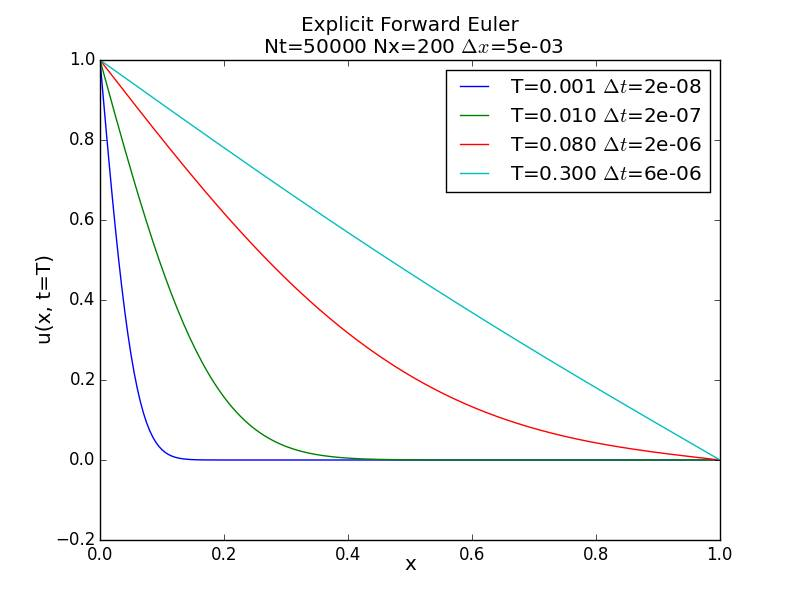
\includegraphics[scale=0.4]{EF_Nt5000_Nx200}
\caption{\label{fig:forward_Euler_u}The concentration of neurotransmitters as a function of position in the synapitc cleft for four different points in time. This results is computed by use of the Forward Euler method. Nt is the number of time steps and Nx is the number of step length.}
\end{center}
\end{figure}

\begin{figure}[!h]
  \begin{minipage}{\linewidth}
    \centering
    \subcaptionbox{\label{fig:backward_Euler_u}Calculated with Backward Euler.}
    {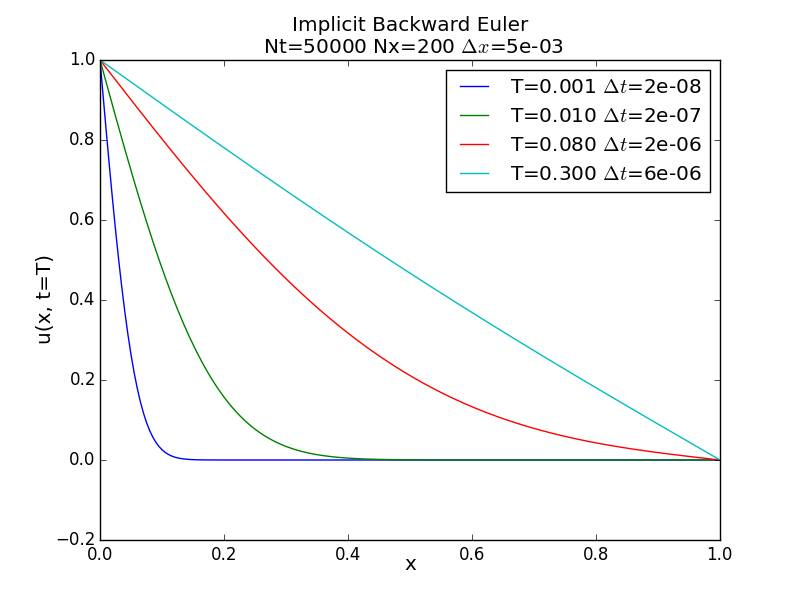
\includegraphics[scale=0.27]{EB_Nt5000_Nx200}}
    \subcaptionbox{\label{fig:Crank_Nicolson_u}Calculated with Crank Nicolson.}
     {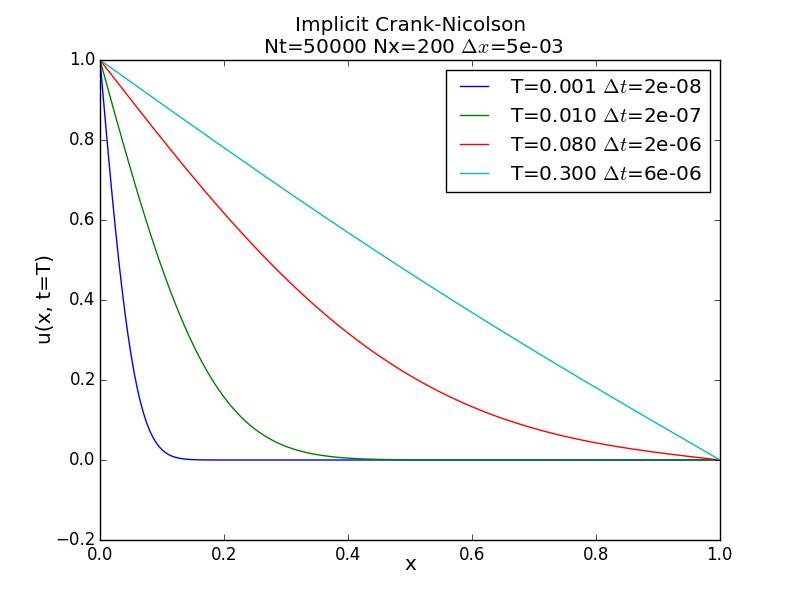
\includegraphics[scale=0.27]{CN_Nt5000_Nx200}}
    \caption{The concentration of neurotransmitters as a function of position in the synapitc cleft for four different points in time. These results are computed by use of the Backward Euler method and the Crank Nicolson scheme. Nt is the number of time steps and Nx is the number of step lengths.}
  \end{minipage}
\end{figure}

\newpage
\subsection{Error in numerical calculated results}
\subsubsection{Relative and absolute global error.}
We know from section \ref{sect:truncation_error} that the spatial local error in the three methods Forward Euler, Backward Euler and Crank Nicolson, are of magnitude $\mathcal{O}(\Delta x^2)$. Although the magnitude of the local error is the same in the three methods, the global error can accumulate to be quite different. We also know that the order of the local error in time is smaller for Crank Nicolson, something that will make the global error less for that method. In Figure \ref{fig:rel_error_all} and \ref{fig:abs_error_all} we can see the relative and absolute error for the three methods, where the absolute error is the absolute value of the difference between the numerically and analytically calculated data. As we would expect, the relative error is linear. This is because we add the same amount of local error in every time step of the algorithm. We can see that the graphs stop to grow when $x$ is approaching $1.0$. This happens most likely because we have made the boundary condition that the density of transmitters is zero in $x=0$. The absolute error is behaving the way we would expect. It starts out in zero because we know the value at the start point, and ends up in zero because we know the value at the endpoint. This results in that the absolute errors are biggest in the middle of the spatial interval.
\begin{figure}[!h]
  \begin{minipage}{\linewidth}
    \centering
    \subcaptionbox{\label{fig:rel_error_all}Relative error.}
    {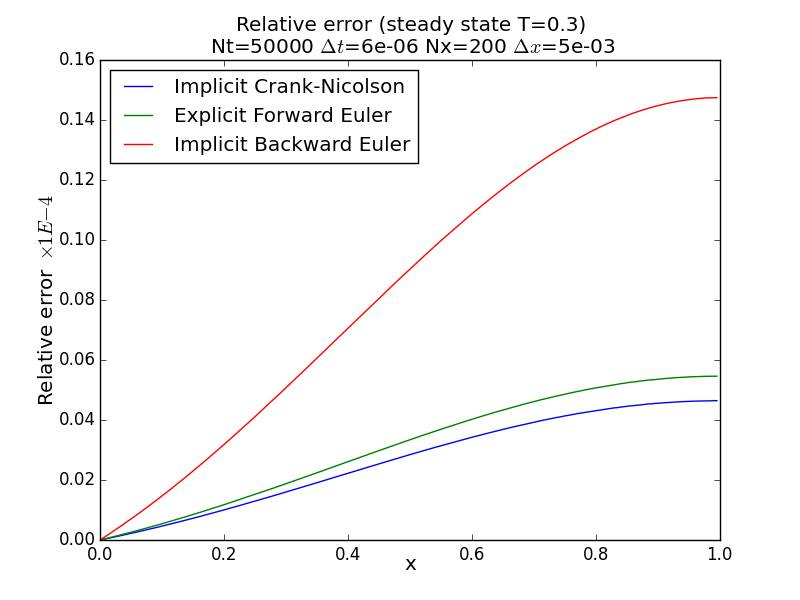
\includegraphics[scale=0.27]{rel_error_all}}
    \subcaptionbox{\label{fig:abs_error_all}Absolute error.}
     {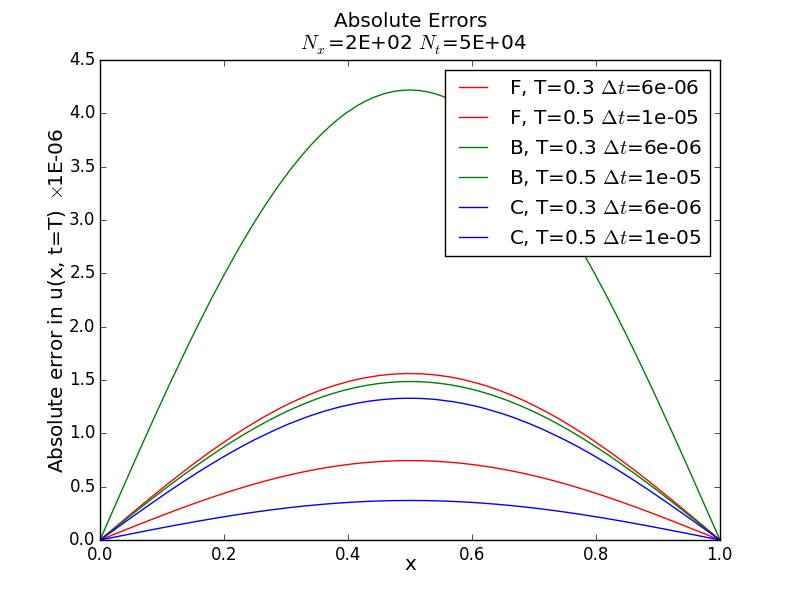
\includegraphics[scale=0.27]{abs_error_all}}
    \caption{The global relative error and the global absolute error of the numerically calculated data, graphed as a function of position in the synaptic cleft. The data are computed by use of Forward Euler method, Backward Euler method and the Crank Nicolson scheme.}
  \end{minipage}
\end{figure}

Plot where restriction is not met\\
- Global error in plot. Bigger for each step.
- Flattens out in top
- Why is the error much less than our calculated error?
- Why does not the global error of t increase?

\newpage
\section{Conclusion}

\section{Comments}

\section{References}
\url{<https://en.wikipedia.org/wiki/Taylor_series>}\\
\url{<https://en.wikipedia.org/wiki/Fourier_series>}\\
\url{<https://en.wikipedia.org/wiki/Tridiagonal_matrix>}\\
\url{<https://en.wikipedia.org/wiki/Toeplitz_matrix>}\\
Mørken

\end{flushleft}
\end{document}















